% !TEX root = ../driver.tex

\begin{textarea}[]
  \only<1>{
    \begin{align*}
      \lim_{n \to \infty} \left( 1+\frac{1}{n} \right)^n
    \end{align*}
  }
  \only<2>{
    What is $e$?
  }
\end{textarea}


\begin{textarea}[]
  \only<1>{
    \begin{align*}
      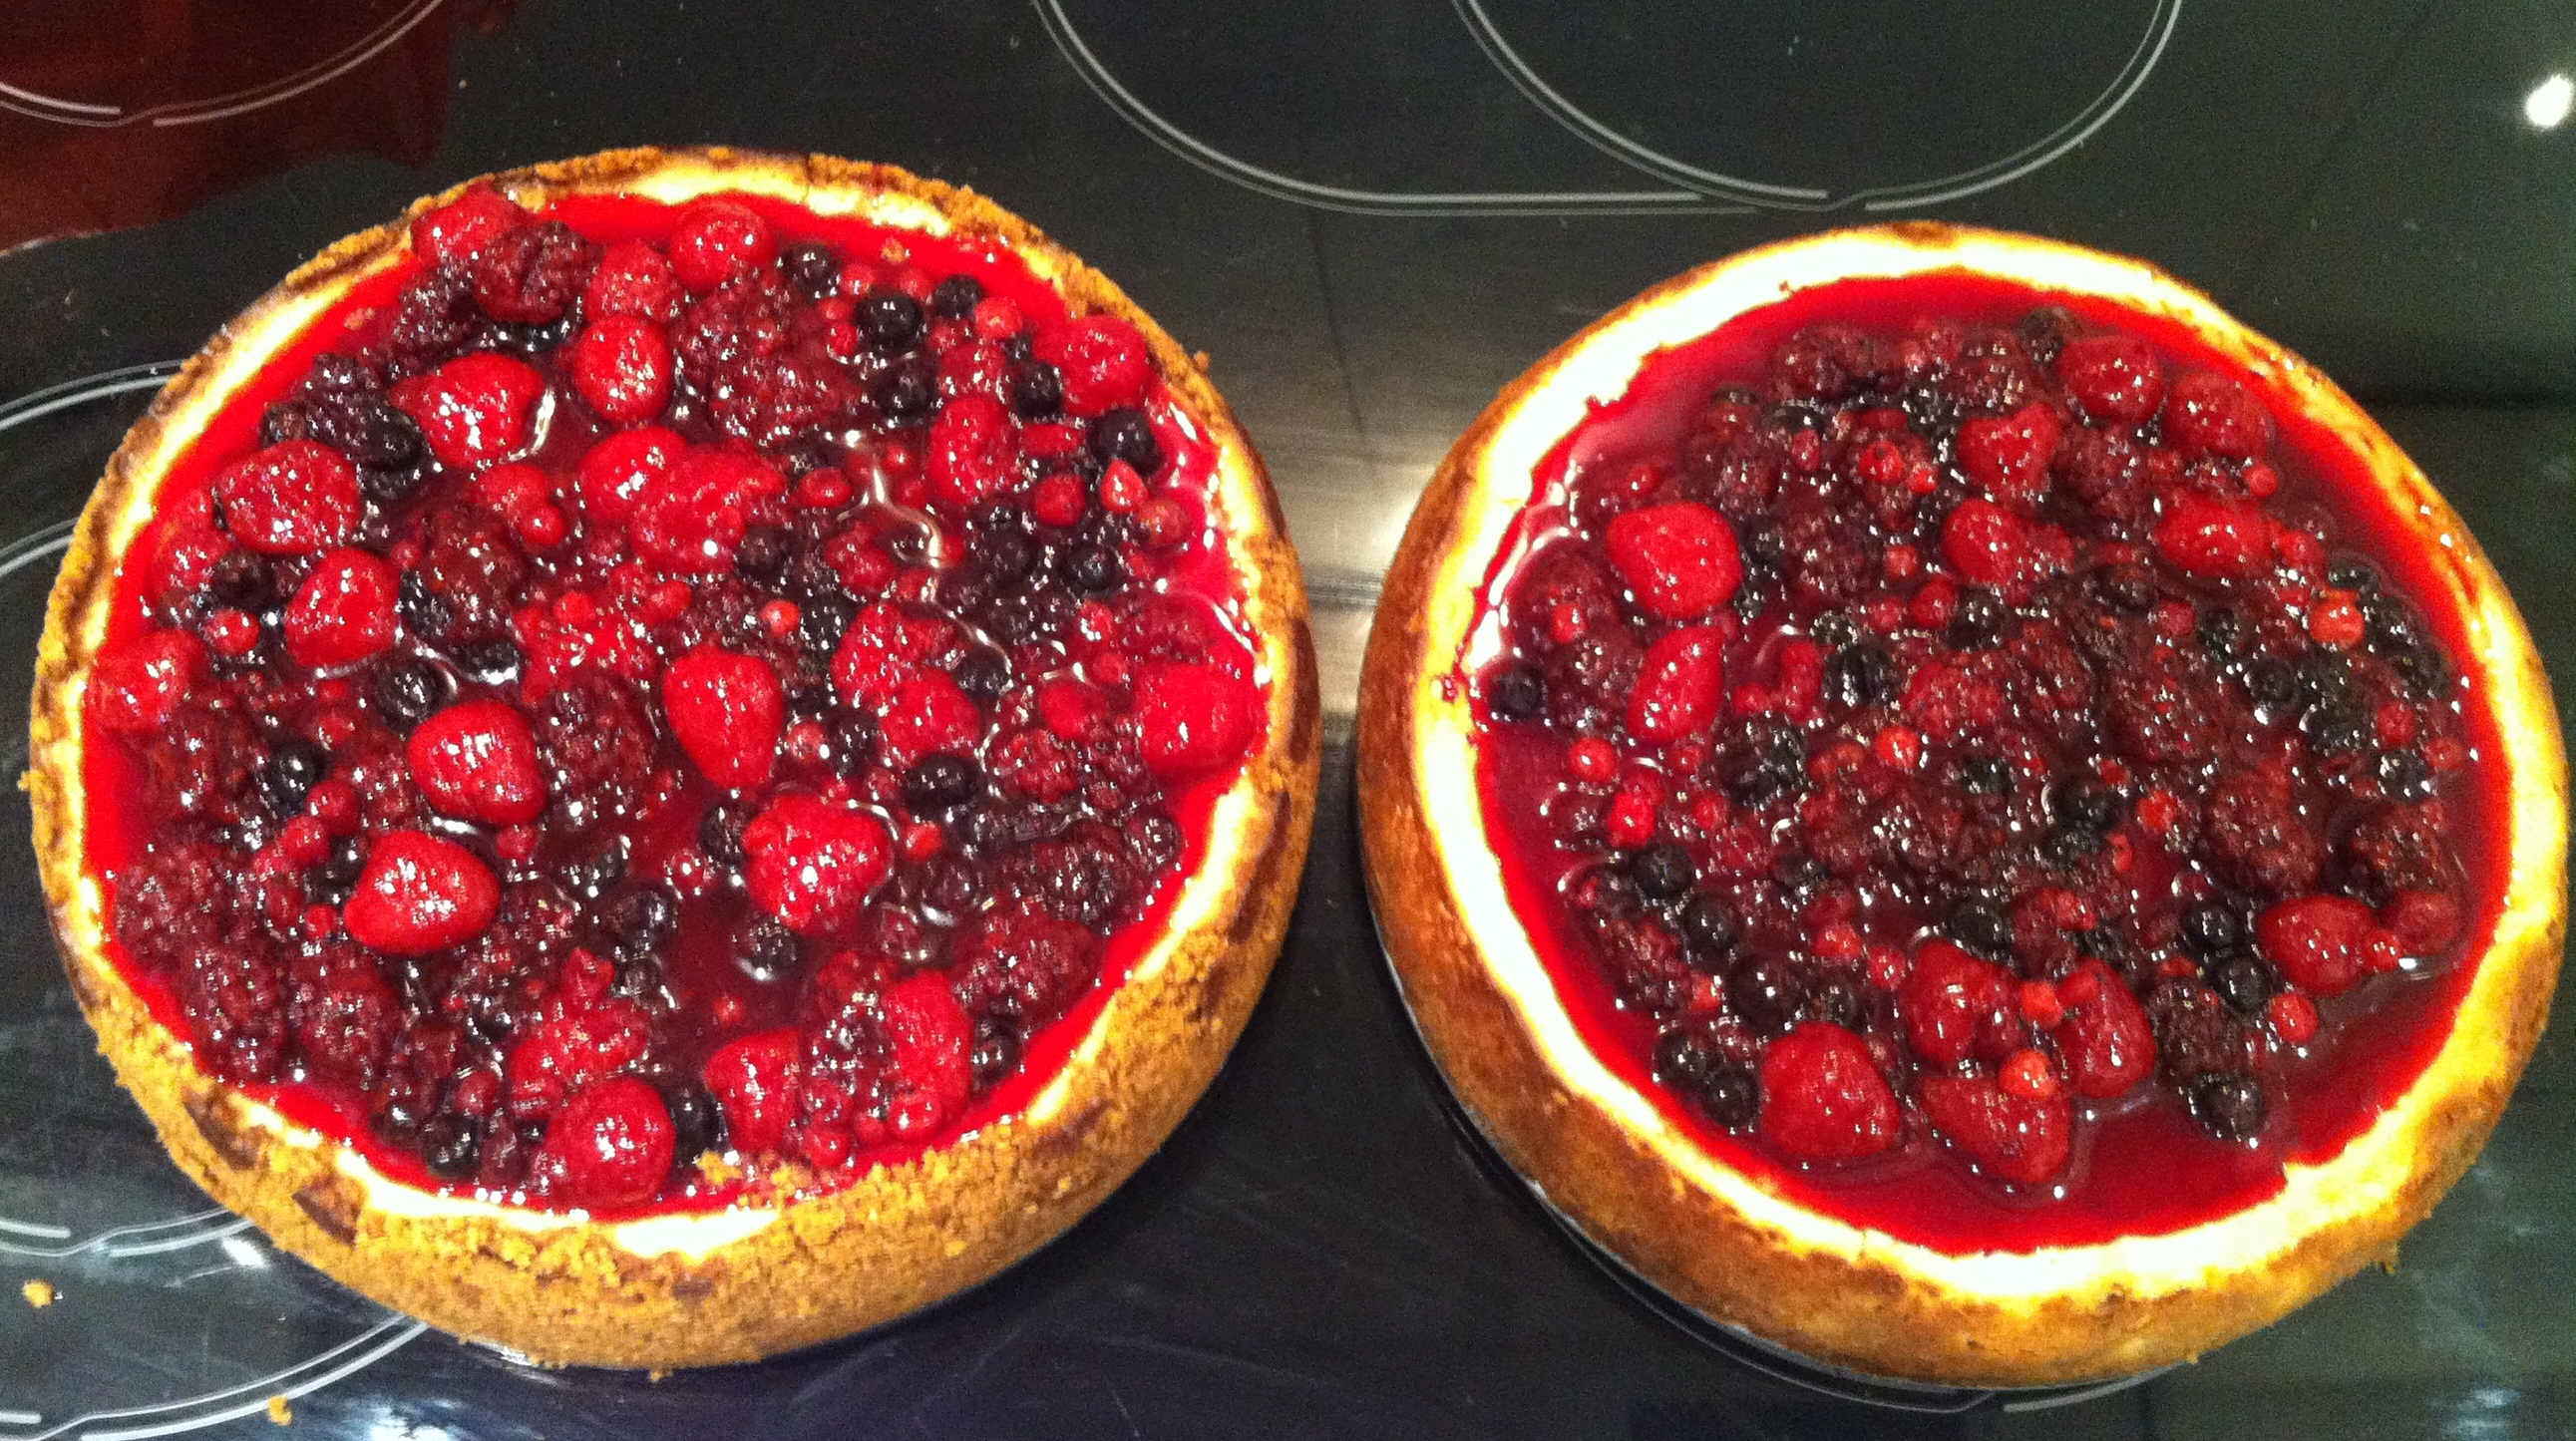
\includegraphics[width=0.5\textwidth]{categories/media/numbers/2pi.jpg}
    \end{align*}
  }
  \only<2>{
    What is $2\pi$
  }
\end{textarea}

% 5
\begin{textarea}[]
  \only<1>{
    \begin{align*}
      \frac{\rho v L}{\eta}
    \end{align*}
  }
  \only<2>{
    What is the Reynolds number?
  }
\end{textarea}

\begin{textarea}[]
  \only<1>{
    \begin{align*}
		e^{i \pi}-1
    \end{align*}
  }
  \only<2>{
	What is zero?
  }
\end{textarea}


\begin{textarea}[]
  \only<1>{
    \begin{align*}
      42
    \end{align*}
  }
  \only<2>{
    What is the answer to the Ultimate Question of Life, the Universe, and Everything?
  }
\end{textarea}


\begin{textarea}[]
  \only<1>{
    \begin{align*}
      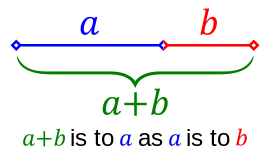
\includegraphics[width=0.5\textwidth]{categories/media/numbers/Golden_ratio_line.png}
      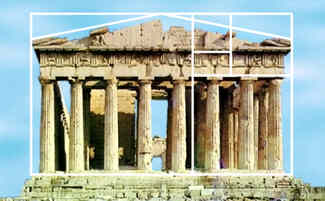
\includegraphics[width=0.5\textwidth]{categories/media/numbers/parthenon-golden-ratio.jpg}
    \end{align*}
  }
  \only<2>{
    What is the Golden Ratio?
  }
\end{textarea}
